\documentclass[12pt,a4paper]{article}

\usepackage{graphicx}
\usepackage{float}
\usepackage{amsmath}
\usepackage{amssymb}
\usepackage{booktabs}
\usepackage{hyperref}

\title{Exploratory Data Analysis Using Python}
\author{
    26M0818 \\
    Department of Computer Science and Engineering \\
    IIT Bombay
}
\date{\today}

\begin{document}

\maketitle

\begin{figure}[H]
    \centering
    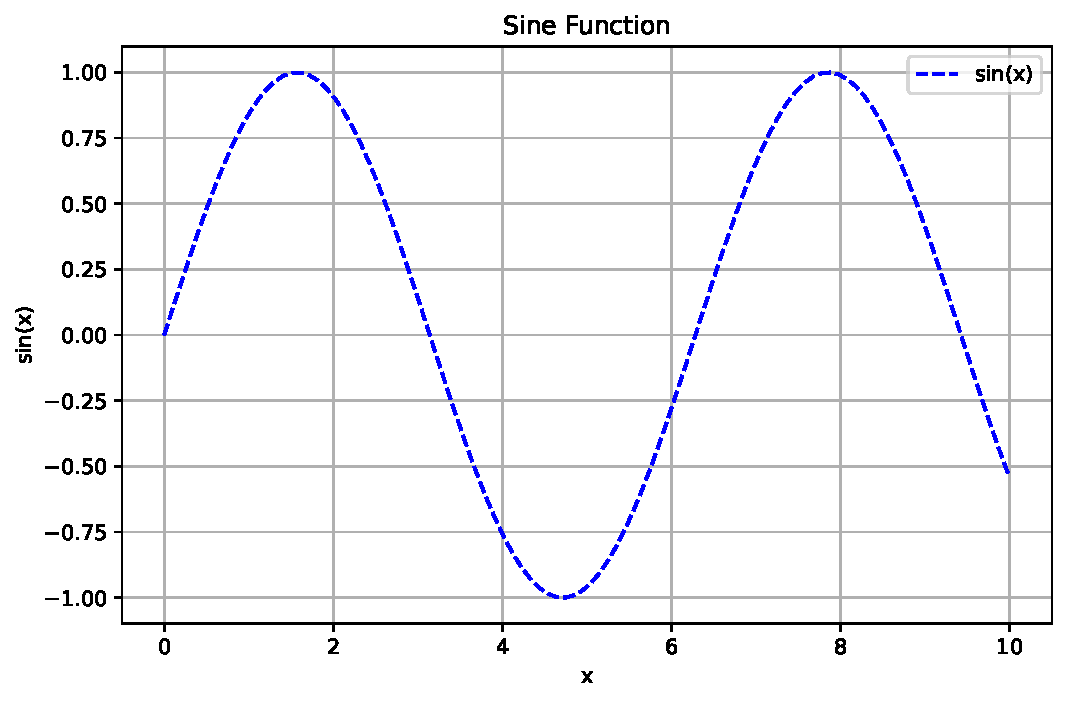
\includegraphics[width=0.7\textwidth]{line_plot.pdf}
    \caption{Random caption}
    \label{fig:line}
\end{figure}
\section{Introduction}

\label{sec:introduction}
Working with some plots for demonstrational purposes.

\subsection{Objectives}
\label{subsec:objectives}
Made some graphs using matplotlib and numpy.

\paragraph{Graphs}
Graphs are genuinely great like \ref{fig:line}.

\section{Text Formatting}
\label{sec:formatting}

Types of texts
\textbf{bold}, \textit{italic},
\underline{underlined}, and
\texttt{monospaced} text.

\noindent{More types of texts \textsc{small capitals}}
and \emph{emphasized text}.

\subsection{Font Sizes}
\label{subsec:fontsizes}

\noindent{\tiny Tiny text}

\noindent{\small Small text}

\noindent{\normalsize Normal text}

\noindent{\Large Large text}

\noindent{\Huge Huge text}

\subsection{Font Families}

This is the default Roman font.

\noindent\textsf{This is sans-serif text.}

\noindent\texttt{This is typewriter text.}

\noindent\textbf{\textit{This is bold and italic.}}

\section{Types of charts}
\label{sec:Types of charts}

\subsection{One}
\begin{itemize}
    \item Line Plot
    \item Bar Chart
    \item Histogram
    \item Scatter Plot
\end{itemize}

\subsection{Two}
\begin{enumerate}
    \item Line Plot
    \item Bar Chart
    \item Histogram
    \item Scatter Plot
\end{enumerate}

\subsection{Three}
\begin{description}
    \item[Line Plot] Shows trends over time.
    \item[Histogram] Shows frequency distributions.
    \item[Scatter Plot] Shows relationships between variables.
\end{description}

\subsection{Four}
\begin{itemize}
    \item A
    \begin{enumerate}
        \item Aa
        \item Ab
    \end{enumerate}

    \item B
    \begin{enumerate}
        \item Ba
        \item Bb
    \end{enumerate}
\end{itemize}


\section{Graphs}
\label{sec:visualization}
Python generated plots.

\subsection{Line Plot}
\label{subsec:line}

\ref{fig:line2} shows the sine function.

\begin{figure}[H]
    \centering
    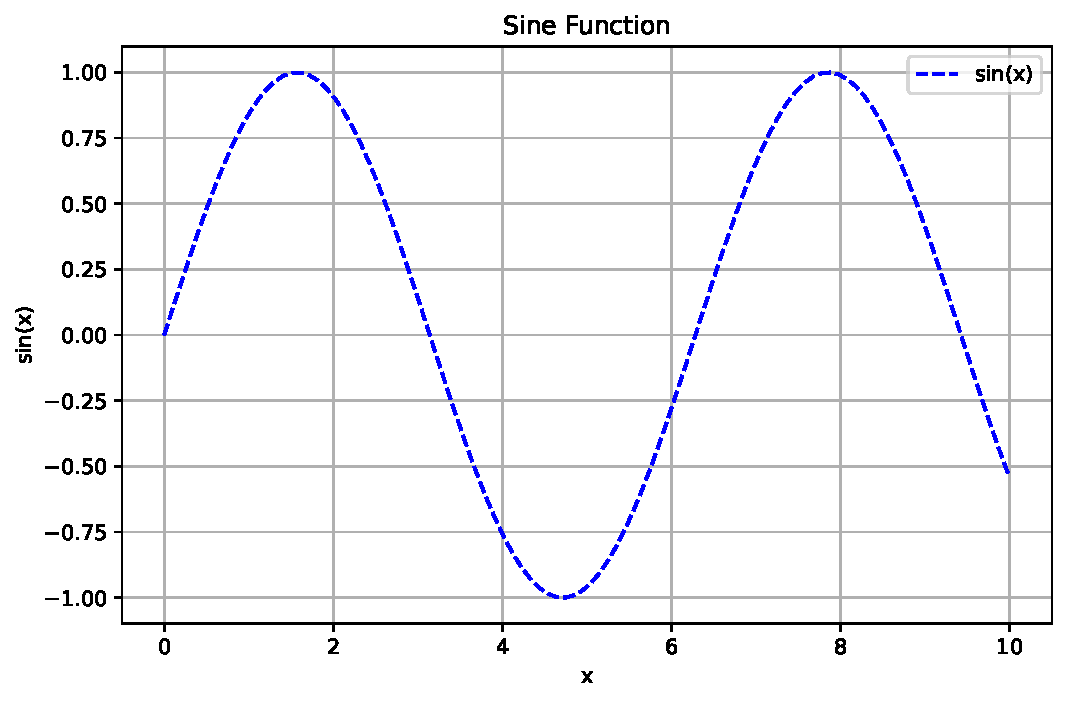
\includegraphics[width=0.7\textwidth]{line_plot.pdf}
    \caption{Line plot of the sine function}
    \label{fig:line2}
\end{figure}

\subsection{Bar Chart}
\label{subsec:bar}

\ref{fig:bar} Random bar chart.

\begin{figure}[H]
    \centering
    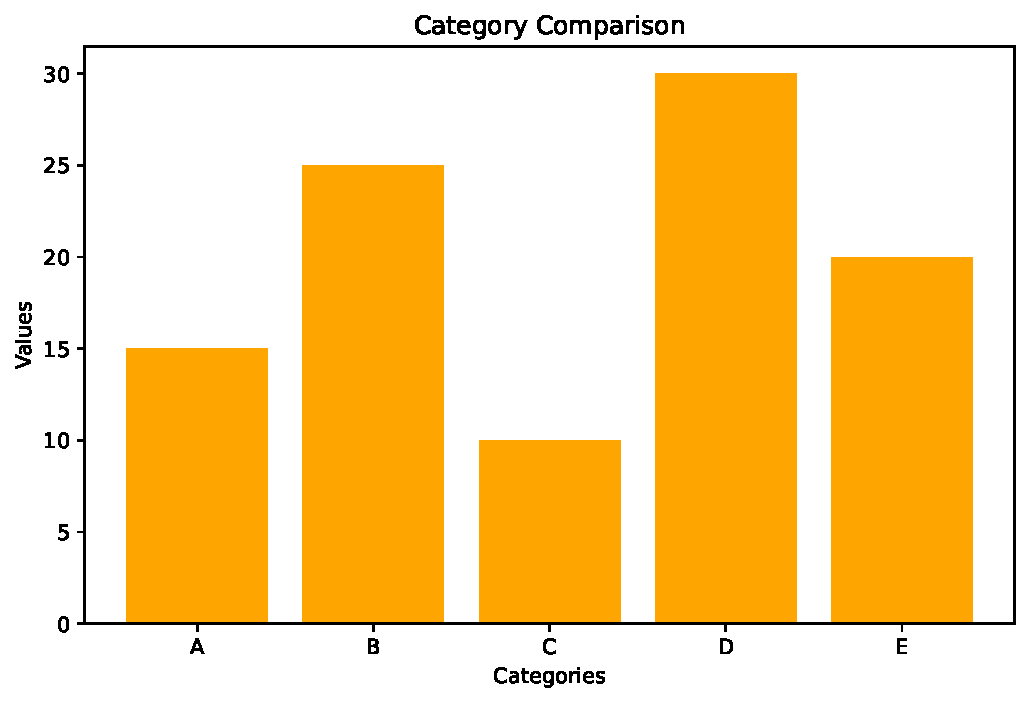
\includegraphics[width=0.7\textwidth]{bar_chart.pdf}
    \caption{Random caption}
    \label{fig:bar}
\end{figure}

\subsection{Histogram}
\label{subsec:histogram}

\ref{fig:histogram} Random Histogram.

\begin{figure}[H]
    \centering
    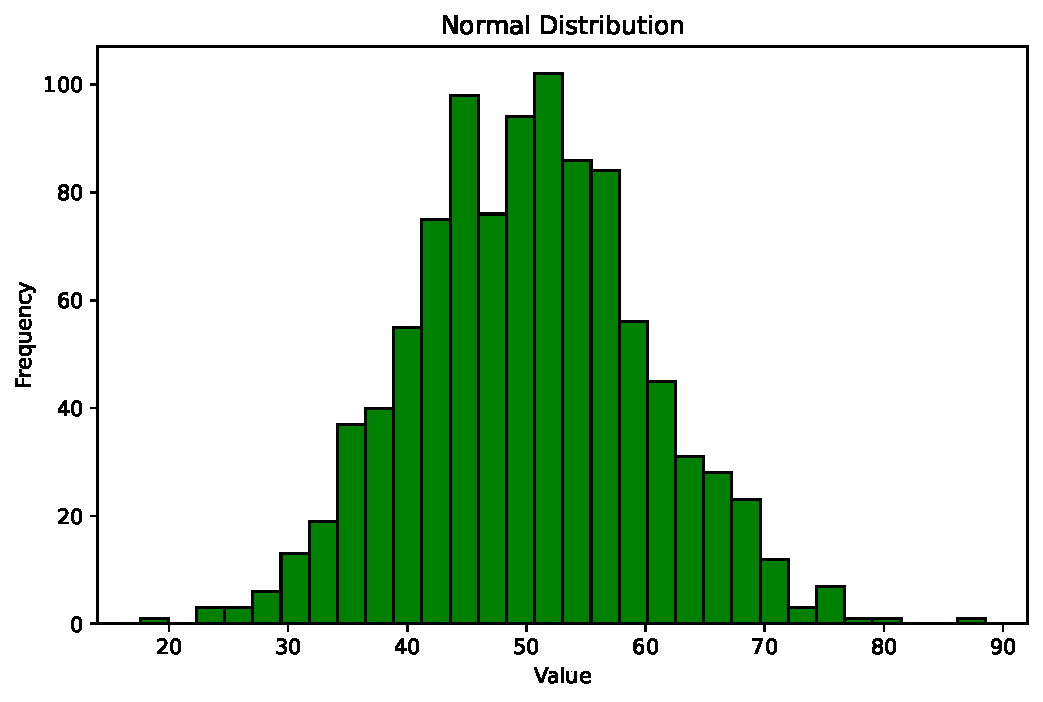
\includegraphics[width=0.7\textwidth]{histogram.pdf}
    \caption{Random caption}
    \label{fig:histogram}
\end{figure}

\subsection{Scatter Plot}
\label{subsec:scatter}

\ref{fig:scatter} Random scatter plot.

\begin{figure}[H]
    \centering
    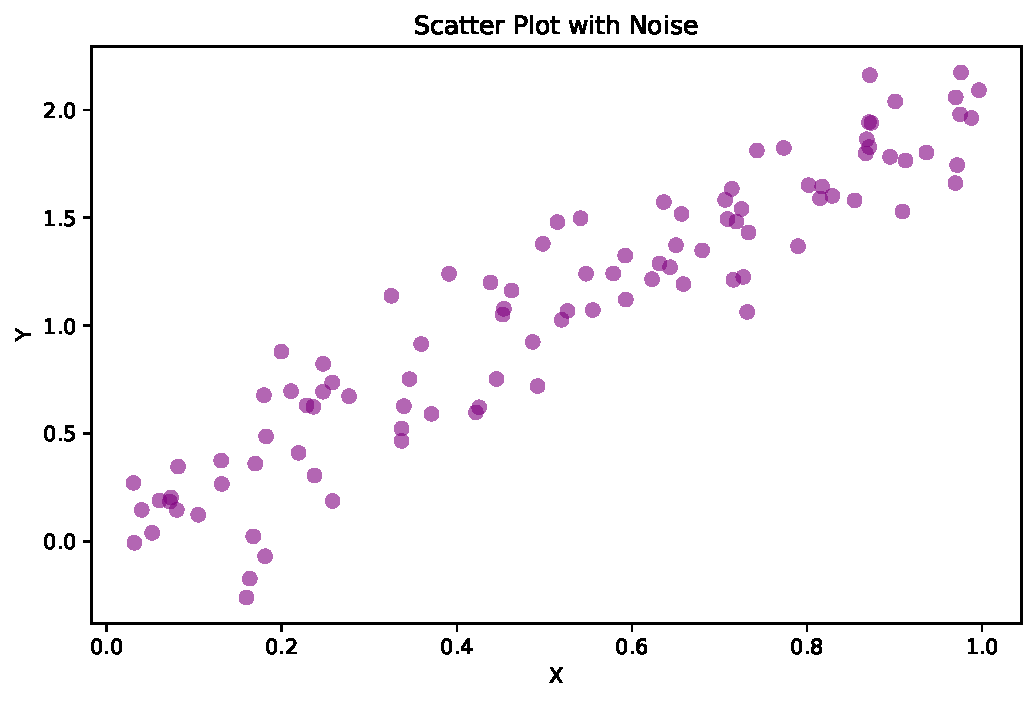
\includegraphics[width=0.7\textwidth]{scatter_plot.pdf}
    \caption{Random caption}
    \label{fig:scatter}
\end{figure}

\section{Complex math stuff}

\subsection{Equations}
Mean: $\mu = \frac{1}{n}\sum_{i=1}^{n}x_i$.

{\centering{Mean but pretty.}}
\begin{equation}
    \mu = \frac{1}{n}\sum_{i=1}^{n}x_i
    \label{eq:mean}
\end{equation}

\subsection{Matrix}

Behold matrix:
\begin{equation}
    A =
    \begin{bmatrix}
        1 & 2 & 3 \\
        4 & 5 & 6 \\
        7 & 8 & 9
    \end{bmatrix}
    \label{eq:matrix}
\end{equation}

\subsection{Multilined equations:}
\begin{equation}
    \begin{aligned}
        f(x) &= x^2 + 2x + 1 \\
             &= (x+1)^2
    \end{aligned}
    \label{eq:derivation}
\end{equation} 

\section*{TANK U}
\end{document}